% !TEX root = ../../main.tex

\subsection{Adsorption isotherms at 77K and room temperature}

Nitrogen sorption isotherms measured at \SI{77}{\kelvin} have been
measured on both powder and \(\rho\)-alumina pellets, with the isotherms
presented in \autoref{shaping:fig:n2adsorption}.
Observation of the physisorption curves sheds light on the
impact of the alumina binder on the materials chosen.
The shapes of all isotherms are visually similar, with the pellet curves
shifted downwards due to the aforementioned structure degradation.
In both powders and pellets, the increased uptake after 0.9 \(p/p^0\)
is a sign of condensation in very large pores or voids, which can
be attributed to intra-pellet spaces and crystal agglomeration.
In the MIL-127(Fe) pellets, a narrow hysteresis curve is seen,
which closes at a \(p/p^0\) of 0.5. This curve corresponds to
capillary condensation in a pore size of around \SI{4}{\nano\metre}.
This pore width is identical to the average pore size of the alumina
binder. However, as this feature is present in both the pellet and 
powder isotherms, it cannot correspond to the binder and is therefore
a consequence of particle agglomeration.

\begin{figure}[p!]
	\centering

	\begin{subfigure}{\linewidth}
		\centering
		\parbox[c]{0.1\linewidth}{\caption{}\label{shaping:fig:n277kuio66}}%
		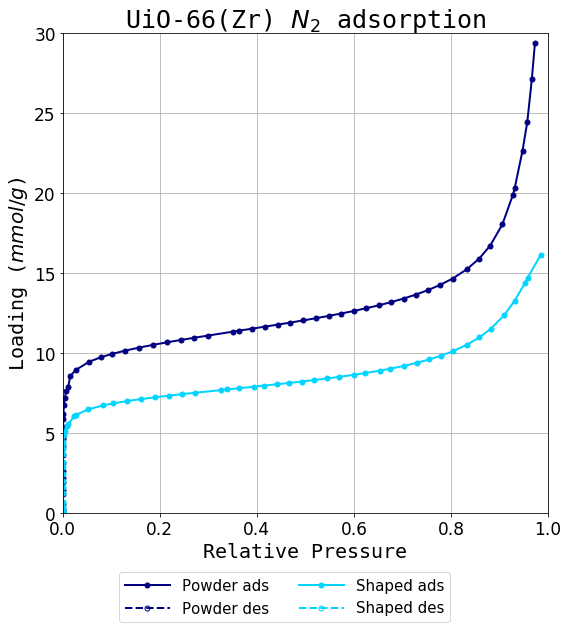
\includegraphics[width=0.35\textwidth]{n277k/UiO-66(Zr)-physisorption}%
		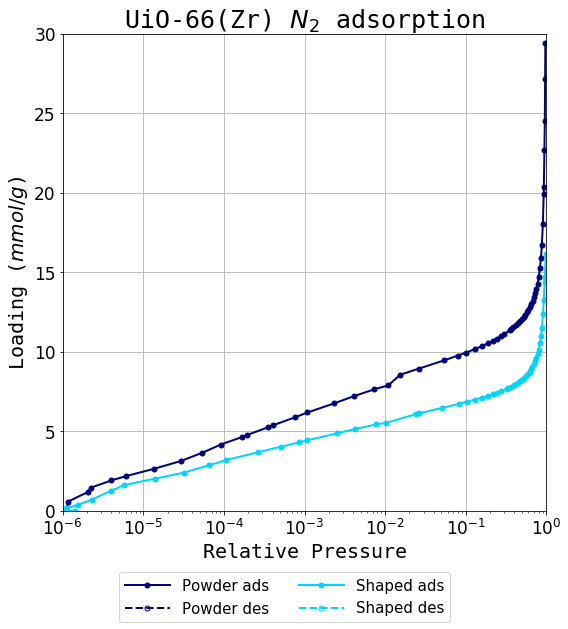
\includegraphics[width=0.35\textwidth]{n277k/UiO-66(Zr)-physisorption-log}%
	\end{subfigure}%

	\begin{subfigure}{\linewidth}
		\centering
		\parbox[c]{0.1\linewidth}{\caption{}\label{shaping:fig:n277kmil100}}%
		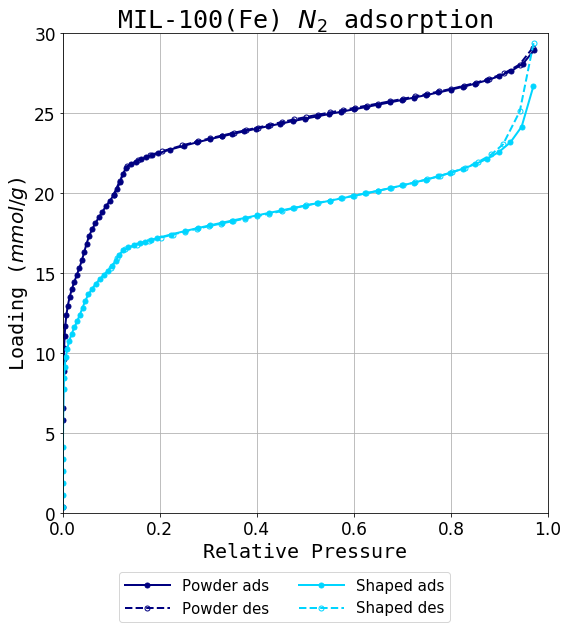
\includegraphics[width=0.35\textwidth]{n277k/MIL-100(Fe)-physisorption}%
		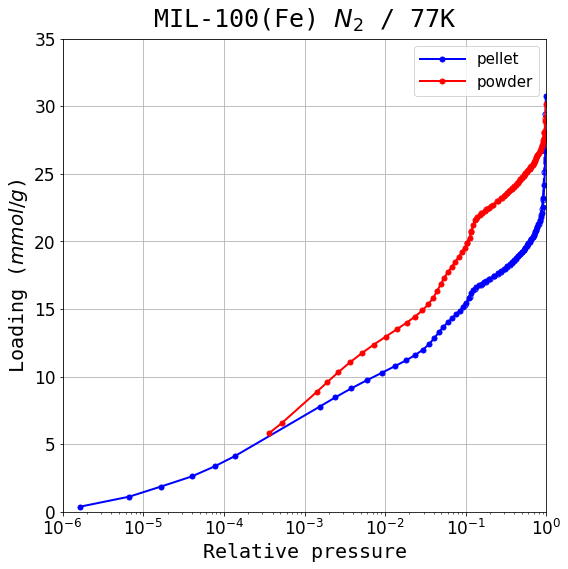
\includegraphics[width=0.35\textwidth]{n277k/MIL-100(Fe)-physisorption-log}%
	\end{subfigure}%

	\begin{subfigure}{\linewidth}
		\centering
		\parbox[c]{0.1\linewidth}{\caption{}\label{shaping:fig:n277kmil127}}%
		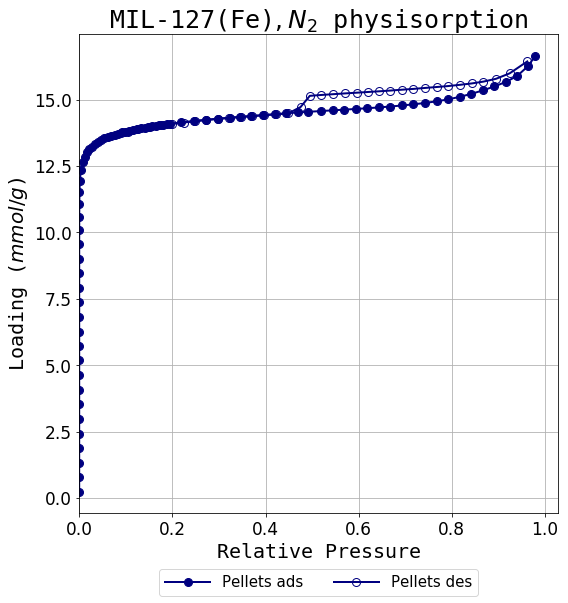
\includegraphics[width=0.35\textwidth]{n277k/MIL-127(Fe)-physisorption}%
		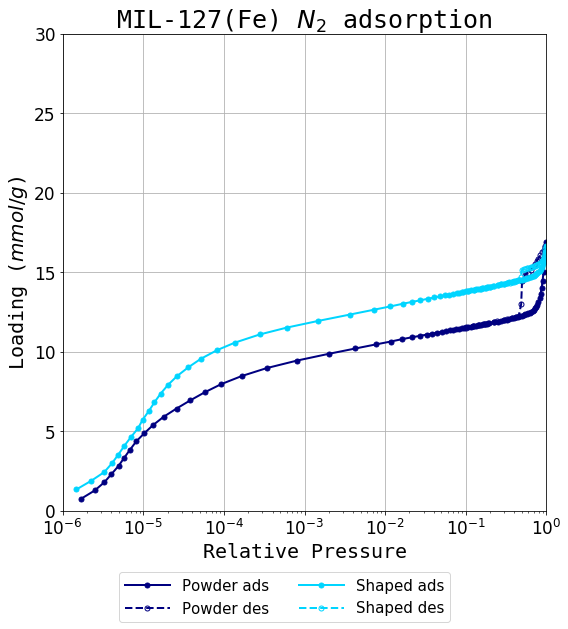
\includegraphics[width=0.35\textwidth]{n277k/MIL-127(Fe)-physisorption-log}%
	\end{subfigure}%

	\caption{Nitrogen isotherms at 77K for (a) UiO-66(Zr),
		(b) MIL-100(Fe) and (c) MIL-127(Fe). The powder sample is in light
		blue while the \(\rho\)-alumina sample in dark blue. Logarithmic
		graphs of the isotherms are on the right for clarity of the low
		pressure region.}%
	\label{shaping:fig:n2adsorption}
\end{figure}

Since no other significant features are visible on the isotherms themselves,
we use pyGAPS to further process them and obtain properties
such as specific surface area, calculated through the BET method and pore
volume, calculated as the volume of nitrogen
adsorbed at a \(p/p^0\) of 0.2.
As the surface area of the binder is lower than the
one of the MOF, a drop in both these properties is expected.
The calculated values are shown in
\autoref{tbl:shaping:propertiestable}.

\begin{table}[htb]
	\centering
	\caption{Properties of the studied powders and pellets}
	\begin{tabular}{lcccc}
		\toprule
		\textbf{MOF}
		                             & \textbf{form}
		                             & \textbf{BET surface area}
		                             & \textbf{Pore volume}
		                             & \textbf{Bulk density}                                                 \\
		                             &                           & (\(m^2/g\)) & (\(cm^3/g\)) & (\(kg/m^3\)) \\
		\midrule
		\multirow{2}{*}{UiO-66(Zr)}  & powder                    & 903         & 0.38         & 0.319        \\
		                             & \(\rho\)-alumina          & 619         & 0.24         & 0.472        \\
		\multirow{2}{*}{MIL-100(Fe)} & powder                    & 1928        & 0.78         & 0.216        \\
		                             & \(\rho\)-alumina          & 1451        & 0.60         & 0.351        \\
		\multirow{2}{*}{MIL-127(Fe)} & powder                    & 1413        & 0.76         & 0.412        \\
		                             & \(\rho\)-alumina          & 1266        & 0.56         & 0.526        \\
		\bottomrule
	\end{tabular}%
	\label{tbl:shaping:propertiestable}
\end{table}%

As predicted, the specific surface area of the shaped samples is
decreased compared to the corresponding powder. While in the case
of MIL-127(Fe) the BET area is only 10\% lower, for the MIL-100(Fe)
and UiO-66(Zr) materials a larger drop is seen, of 25\% and 31\%,
respectively.
A similar decrease can be seen in total pore volume,
with a 36\%, 23\% and 26\% loss seen
in UiO-66(Zr), MIL-100(Fe) and MIL-127(Fe) respectively.
The decrease in both surface area and micropore volume is
too large for it to be a consequence of the presence of non-porous binder.
It is therefore theorised that some structure degradation must have
occurred during the pelletisation process.
Despite a loss in surface area, the bulk density of the material
has increased, due to crystal aggregation.